\hypertarget{context-and-scope}{%
\section{Context and Scope}\label{context-and-scope}}

The \textbf{GPS\_Tracker} set of projects intended to be used for the
optimization of mobile users' signals. Optimization aims to find the
best positions for the base stations represented by the UAVs.

\hypertarget{business-context}{%
\subsection{Business context}\label{business-context}}

\begin{figure}
\centering
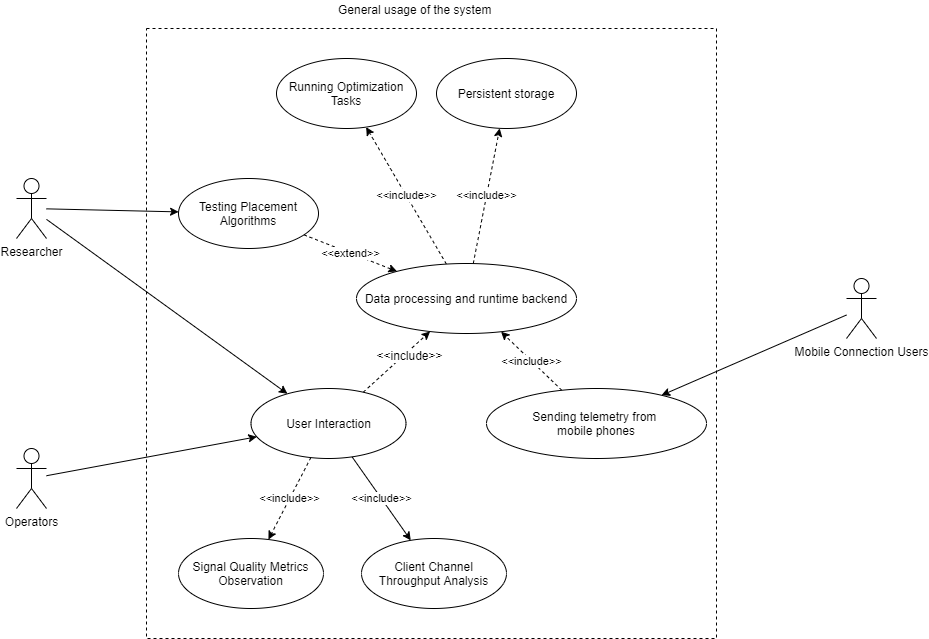
\includegraphics{schemes/use-case/Main-Usage-Use-Case.png}
\caption{Business context representation}
\end{figure}

There are three types of actors:

\begin{enumerate}
\def\labelenumi{\arabic{enumi}.}
\tightlist
\item
  Mobile Connection Users - the volunteers that allowed to install the
  special software GPS\_Android on their mobile phones. They are
  connected to the access points provided by the network which
  efficiency we seek to increase.
\item
  Operators - the owners of the mobile network who are interested in the
  increased network throughput. They want to optimize either technical
  characteristics of the radio technologies or optimize the layout of
  the access points.
\item
  Researchers - scientific guys who want to test the layout optimization
  algorithms on the telemetry data from mobile connection users. They
  also can consult Operators what how to exactly treat the information
  provided by \textbf{GPS\_Tracker}.
\end{enumerate}

Also, that is worth describing the activities performing in the system.
There are three important use-cases:

\begin{enumerate}
\def\labelenumi{\arabic{enumi}.}
\tightlist
\item
  User interaction - There is a web application that allows users to
  interact with the backend to fetch and observe information stored.
  Also, there is a purpose to filter data and run optimization tasks.
\item
  Sending telemetry data from mobile phones - each mobile connection
  user has a special program installed on the phones. That is an
  important part of the software because it provides the real info on
  the radio network quality attributes.
\item
  Data processing and runtime backend - There is a set of the program
  running in the backend that performs a lot of processing operations to
  serve the user requests. No direct interaction from the actors
  required.
\end{enumerate}

Also, there are other activities included in or to extend these three
use-cases:

\begin{longtable}[]{@{}ll@{}}
\caption{Main use-cases description}\tabularnewline
\toprule
\begin{minipage}[b]{0.31\columnwidth}\raggedright
Use-case\strut
\end{minipage} & \begin{minipage}[b]{0.63\columnwidth}\raggedright
Description\strut
\end{minipage}\tabularnewline
\midrule
\endfirsthead
\toprule
\begin{minipage}[b]{0.31\columnwidth}\raggedright
Use-case\strut
\end{minipage} & \begin{minipage}[b]{0.63\columnwidth}\raggedright
Description\strut
\end{minipage}\tabularnewline
\midrule
\endhead
\begin{minipage}[t]{0.31\columnwidth}\raggedright
Signal Quality Metrics Observation\strut
\end{minipage} & \begin{minipage}[t]{0.63\columnwidth}\raggedright
Each telemetry message from the mobile connection users includes
information about the location and current wireless connection RSS. That
information is shown via different figures available in the UI.\strut
\end{minipage}\tabularnewline
\begin{minipage}[t]{0.31\columnwidth}\raggedright
Client Channel Throughput Analysis\strut
\end{minipage} & \begin{minipage}[t]{0.63\columnwidth}\raggedright
Each client performs uplink and downlink throughput evaluation. These
throughput evaluation drawn are to be observed and analyzed in
**GPS\_Frontend*.\strut
\end{minipage}\tabularnewline
\begin{minipage}[t]{0.31\columnwidth}\raggedright
Testing Placement Algorithms\strut
\end{minipage} & \begin{minipage}[t]{0.63\columnwidth}\raggedright
There is a simple and extensible approach on how to add additional
optimization algorithms to test. There is a unified interface to access
telemetry data.\strut
\end{minipage}\tabularnewline
\begin{minipage}[t]{0.31\columnwidth}\raggedright
Running Optimization Tasks\strut
\end{minipage} & \begin{minipage}[t]{0.63\columnwidth}\raggedright
\textbf{GPS\_Tracker} can run several optimizations in parallel. The
researches can compare the results of different algorithms.\strut
\end{minipage}\tabularnewline
\begin{minipage}[t]{0.31\columnwidth}\raggedright
Persistent storage\strut
\end{minipage} & \begin{minipage}[t]{0.63\columnwidth}\raggedright
The telemetry from the users as well as optimization task results are
saved persistently in well-known JSON format. Further, the data can be
imported in other analytic tools.\strut
\end{minipage}\tabularnewline
\bottomrule
\end{longtable}

\hypertarget{technical-context}{%
\subsection{Technical context}\label{technical-context}}

The following diagrams show the input/output interfaces for the main
components.

\begin{figure}
\centering
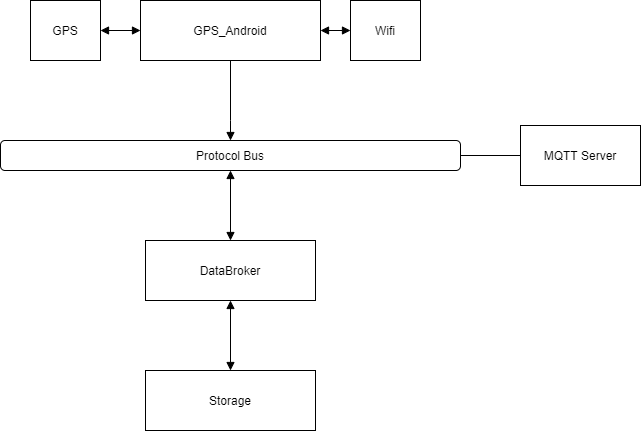
\includegraphics[width=0.5\textwidth,height=\textheight]{schemes/architecture/ArchitectureDiagram.png}
\caption{Abstract Architecture representation}
\end{figure}
